\documentclass[10pt]{beamer}
\usetheme[]{Feather}
\setbeamercolor{Feather}{fg=black!20,bg=black}
\setbeamercolor{structure}{fg=black}
\usepackage[utf8]{inputenc}
\usepackage[spanish]{babel}
\usepackage[T1]{fontenc}
\usepackage{helvet}
\usepackage{lipsum}
\usepackage{amsmath,amssymb,amsfonts}
\usepackage{amsthm}
\usepackage{physics}
\usepackage{framed, color}
\usepackage{epsfig}
\usepackage{acronym}
\usepackage{multirow, array} 
\usepackage{float}
\usepackage[T1]{fontenc}
\usepackage{natbib}
\usepackage{fancyhdr}
\usepackage{xcolor}
\usepackage{multicol}
\usepackage{mdframed}
\usepackage{endnotes}
\usepackage{listings}
\usepackage{tensor}
\usepackage{csquotes}
\renewcommand{\thefootnote}{\arabic{footnote}}
\newcommand{\chref}[2]{
  \href{#1}{{\usebeamercolor[bg]{Feather}#2}}
}
\title[Regresión Logística]
{
      \textbf{Regresión Logística}
}

\subtitle[ - Clasifiación]
{Reconocimiento de Patrones}

\author[Dr. Gamaliel ]
{      Dr. Gamaliel Moreno Chávez  \\ \href{mailto:me@example.com}{gamalielmch@uaz.edu.mx} 
}

\institute[]
{
      \large{Maestría en Ciencias del Procesamiento de la Información}\\
      Universidad Autónoma de Zacatecas
  
  %there must be an empty line above this line - otherwise some unwanted space is added between the university and the country (I do not know why;( )
}
\date{Enero-Julio 2021}
\begin{document}

%%%%%%%%%%%%%%%%%%%%%%%%%%%%%%%%%%%%%
{\1% % this is the name of the PDF file for the background
\begin{frame}[plain,noframenumbering] % the plain option removes the header from the title page, noframenumbering removes the numbering of this frame only
  \titlepage % call the title page information from above
\end{frame}}
%%%%%%%%%%%%%%%%%%%%%%%%%%%%%%%%%%%%%
\begin{frame}{Temas}
\tableofcontents
\end{frame}
%%%%%%%%%%%%%%%%%%%%%%%%%%%%%%%%%%%%%
\section{Clasificación}
\subsection{Clasificación}
\begin{frame}
  \frametitle{Clasificación}
  \begin{itemize}
   \item Regresión: $y=h_{\boldsymbol{\theta}} (\boldsymbol{x})$ con $y\in \mathbb{R}$ continuo
   \item Clasificación: $y=h_{\boldsymbol{\theta}} (\boldsymbol{x})$ como antes, pero con $y \in \mathbb{C}$ es discreto y posiblemente no ordenado.
   
   \item iniciaremos con problema de clasificación binario $y\in \lbrace 0,1\rbrace$
   \item Ejemplos 
   \begin{itemize}
   \item Clasificación de correo como spam o no spam
   \item Paciente con enfermedad o no la presenta
   \item Una máquina fallará o no dadas ciertas lecturas de sensores
   \end{itemize}
   \item Dado $ \boldsymbol{x}^{(i)}$, el valor deseado correspondiente  $y^{i}$ se llama etiqueta
  \end{itemize}
\end{frame}
%%%%%%%%%%%%%%%%%%%%%%%%%%%%%%%%%%%%%
\subsection{Regresión Logística}
\begin{frame}
  \frametitle{Regresión Logística}
   \begin{itemize}
   \item Buscar una hipótesis $h(\boldsymbol{x})\in \left[ 0, 1\right] $
   \item Elijamos: 
   \begin{equation*}
   h_{\boldsymbol{\theta}} = g(\boldsymbol{\theta}^T \boldsymbol{x})= \sigma (\boldsymbol{\theta}^T \boldsymbol{x})= \frac{1}{1+e^{-\boldsymbol{\theta}^T \boldsymbol{x}}} 
   \end{equation*}
   con $g$ una función no lineal, es este caso concreto elegido como la función sigmoide, función logística
   \end{itemize}


\begin{center}
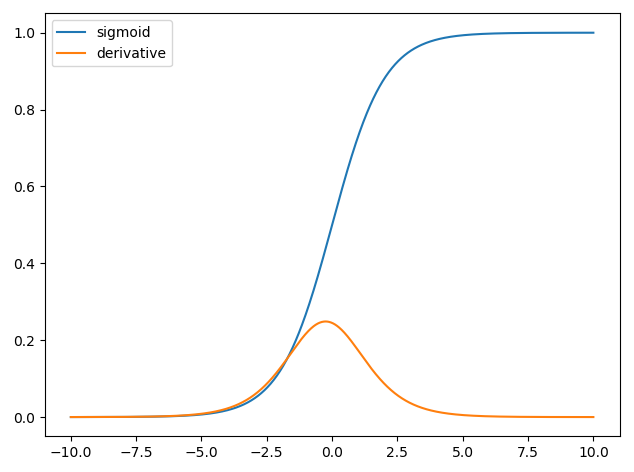
\includegraphics[scale=0.3]{im1.png}
\end{center}   
   Función logística $\sigma(z)= \frac{1}{1+e^{-z}}$ y su derivada $\sigma ' (z)= \sigma(z)(1-\sigma(z))$
\end{frame}
%%%%%%%%%%%%%%%%%%%%%%%%%%%%%%%%%%%%%

\begin{frame}
\frametitle{Regresión Logística. Planteo probabilístico}
\begin{itemize}
\item Vamos a usar planteo probabilístico para derivar solución 
\item Supongamos que la hipótesis cumple
\begin{equation*}
P(y=1\vert \boldsymbol{x};\boldsymbol{\theta} )= h_{\boldsymbol{\theta}} (\boldsymbol{x})
\end{equation*}
además
\begin{equation*}
P(y=0\vert \boldsymbol{x};\boldsymbol{\theta} )= 1- h_{\boldsymbol{\theta}} (\boldsymbol{x})
\end{equation*}
las cuales se pueden combinar (Bernoulli)
\begin{equation*}
P(y \vert \boldsymbol{x};\boldsymbol{\theta} )= h_{\boldsymbol{\theta}} (\boldsymbol{x})^y(1- h_{\boldsymbol{\theta}} (\boldsymbol{x}))^{1-y}
\end{equation*}
\item La verosimilitud, igual que el caso de regresión con i.i,d es:

\begin{equation*}
L(\boldsymbol{\theta})= P(\boldsymbol{y} \vert \boldsymbol{X};\boldsymbol{\theta} )= \prod_{i=1}^{m} P(y^{(i)}\vert \boldsymbol{x}^{(i)};\boldsymbol{\theta} )  
\end{equation*}
\begin{equation*}
=\prod_{i=1}^{m} h_{\boldsymbol{\theta}} (\boldsymbol{x}^{(i)})^{y^{(i)}}( 1- h_{\boldsymbol{\theta}} (\boldsymbol{x}^{(i)}))^{1-y^{(i)}}
\end{equation*}
\end{itemize}

\end{frame}

%%%%%%%%%%%%%%%%%%%%%%%%%%%%%%%%%%%%%
\begin{frame}
\frametitle{Regresión Logística. Planteo probabilístico}
\begin{itemize}
\item Queremos maximizar esta verosimilitud, lo que es más fácil a través de la verosimilitud logarítmica
\begin{equation*}
\begin{split}
\ell (\boldsymbol{\theta})= ln L(\boldsymbol{\theta}) & = \sum_{i=1}^{m} ln \left( h_{\boldsymbol{\theta}} (\boldsymbol{x}^{(i)})^{y^{(i)}}( 1- h_{\boldsymbol{\theta}} (\boldsymbol{x}^{(i)}))^{1-y^{(i)}} \right) \\
 & = \sum_{i=1}^{m} y^{(i)}ln \left( h_{\boldsymbol{\theta}}  (\boldsymbol{x}^{(i)})\right) + (1-y^{(i)}) ln ( 1- h_{\boldsymbol{\theta}} (\boldsymbol{x}^{(i)}))
\end{split} 
\end{equation*}
\item Podemos maximizar esto utilizando ascenso de gradiente:
\begin{equation*}
\boldsymbol{\theta} \leftarrow \boldsymbol{\theta} + \alpha \nabla_{\boldsymbol{\theta}} \ell (\boldsymbol{\theta})
\end{equation*}
\item Si derivamos $\partial \ell (\boldsymbol{\theta})/ \partial \theta_j$ llegamos con $\sigma ' (z)= \sigma(z)(1-\sigma(z))$ a

\begin{equation*}
\frac{\partial}{\partial \theta_j} \ell (\boldsymbol{\theta})= \sum_{i=1}^{m}  \left( y^{(i)}- h_{\boldsymbol{\theta}} (\boldsymbol{x}^{(i)}) \right) \boldsymbol{x}^{(i)}_{j} \quad  \nabla_{\boldsymbol{\theta}} \ell (\boldsymbol{\theta})=  \sum_{i=1}^{m} \left( y^{(i)}- h_{\boldsymbol{\theta}} (\boldsymbol{x}^{(i)}) \right) \boldsymbol{x}^{(i)}
\end{equation*}

\end{itemize}
\end{frame}
%%%%%%%%%%%%%%%%%%%%%%%%%%%%%%%%%%%%%

\begin{frame}
\frametitle{Regresión Logística. Planteo probabilístico}
\begin{itemize}
\item Con lo anterior obtenemos para el ascenso estocástico de gradiente:
\begin{equation*}
\theta_{j} \leftarrow \theta_{j} + \alpha \left( y^{(i)}- h_{\boldsymbol{\theta}} (\boldsymbol{x}^{(i)}) \right) \boldsymbol{x}^{(i)}_{j} \quad  \boldsymbol{\theta}\leftarrow \boldsymbol{\theta} + \alpha \left( y^{(i)}- h_{\boldsymbol{\theta}} (\boldsymbol{x}^{(i)}) \right) \boldsymbol{x}^{(i)}
\end{equation*}
\item  Es exactamente la misma expresión que para los mínimos cuadrados ordinarios (OLS), a pesar de que $ h_{\boldsymbol{\theta}}(\cdot)$ es distinta
\end{itemize}
\end{frame}
%%%%%%%%%%%%%%%%%%%%%%%%%%%%%%%%%%%%%
\section{Modelos lineales generalizados}
\subsection{Familia exponencial}
\begin{frame}
  \frametitle{Modelos lineales generalizados}
  \begin{itemize}
  \item Hemos visto dos tipos de problemas
  \begin{itemize}
  \item Regresión lineal con mínimos cuadrados: $y\vert \boldsymbol{x};\boldsymbol{\theta} \backsim \mathcal{N}(\boldsymbol{\mu} \sigma^2)$
  \item Regresión logística:  $y\vert \boldsymbol{x};\boldsymbol{\theta} \backsim Ber(\phi)$
  \end{itemize}
  \item ¿Por qué en ambos problemas llegamos a la misma regla de actualización de $\boldsymbol{\theta}$: 
       \begin{equation*}
        \boldsymbol{\theta}\leftarrow \boldsymbol{\theta} + \alpha \left( y^{(i)}- h_{\boldsymbol{\theta}} (\boldsymbol{x}^{(i)}) \right) \boldsymbol{x}^{(i)} \text{  ?}
       \end{equation*}
       \item Ambos métodos pertenecen a los Modelos Lineales Generalizados (GLM)
  \end{itemize}
\end{frame}
%%%%%%%%%%%%%%%%%%%%%%%%%%%%%%%%%%%%% 

\begin{frame}
  \frametitle{Familias de distribuciones}
  \begin{itemize}
  \item Podemos ver las distribuciones con sus parámetros como familias:
   \begin{itemize}
   \item $Ber(\phi): P(y=1; \theta)= \theta$
   \item $\mathcal{N}(\boldsymbol{\mu}, \sigma^2): p(x; \mu , \sigma)= \frac{1}{\sqrt{2\pi \sigma}} e^{-\frac{1}{2}\left( \frac{x-\mu}{\sigma} \right)^2}$
   \end{itemize}
   \item Esto es: cada instancia de parámetros produce una distribución particular
   \item Mostraremos que estos son casos especiales de la familia exponencial 
  \end{itemize}
\end{frame}
%%%%%%%%%%%%%%%%%%%%%%%%%%%%%%%%%%%%% 
\begin{frame}
  \frametitle{La familia exponencial}
  \begin{itemize}
  \item La familia exponencial incluye las distribuciones que se pueden expresar:
  \begin{equation*}
  p(y;\boldsymbol{\eta})= b(y)exp(\boldsymbol{\eta}^T \boldsymbol{T}(y)-a(\boldsymbol{\eta}))
  \end{equation*}
  \item $\boldsymbol{\eta}$ es el parámetro natural (o canónico) de la distribución
  \item $\boldsymbol{T}(y)$ es el estadístico suficiente. En casos aquí, se cumple $\boldsymbol{T}(y)=y$
  \item $a(\boldsymbol{\eta})$ es la función de partición logarítmica
  \item Usualmente $e^{-a(\boldsymbol{\eta})}$ es constante de normalización 
  \item Elección fija de $\boldsymbol{T}, a$ y $b$ define una familia (o conjunto) de distribuciones parametrizadas con $ \boldsymbol{\eta}$
  \end{itemize}
\end{frame}
%%%%%%%%%%%%%%%%%%%%%%%%%%%%%%%%%%%%%

\begin{frame}
  \frametitle{Caso de distribución de Bernoulli}
\begin{flushright}$p(y;\boldsymbol{\eta})= b(y)exp(\boldsymbol{\eta}^T \boldsymbol{T}(y)-a(\boldsymbol{\eta})) $ \end{flushright}
Distribución de Bernoulli  
\begin{equation*}
\begin{split}
p(y;\phi)&= \phi^y (1-\phi)^{1-y}= exp(ln(\phi^y (1-\phi)^{1-y}))\\
&= exp(y ln\phi + (1-y)ln(1-\phi))\\
& = exp \left( 	 \underbrace{\left(ln  \left(  \frac{\phi}{1-\phi}\right)  \right) }_{\eta}   \underbrace{y}_{\boldsymbol{T}(y)} + \underbrace{ln(1-\phi)}_{-a(\boldsymbol{\eta})}  \right) 
\end{split}
\end{equation*}  
  con lo que se deriva  el parámetro natural
  \begin{equation*}
  \boldsymbol{\eta}= \eta=ln  \left(  \frac{\phi}{1-\phi}\right) 
  \end{equation*}
\end{frame}
%%%%%%%%%%%%%%%%%%%%%%%%%%%%%%%%%%%%%
\begin{frame}
  \frametitle{Caso de distribución de Bernoulli}
  \begin{itemize}
  \item Despejando $\phi$ en términos de $\eta$ resulta en:
  \begin{equation*}
  \phi= \frac{e^\eta}{1+e^\eta}= \frac{1}{1+e^{-\eta}}
  \end{equation*}
  es la función logística que usamos anteriormente
  \item Además
  \begin{align*} 
  T(y)&=y\\ 
  a(\eta)&=-ln(1-\phi)=ln(1+e^\eta)\\ 
  b(y)&=1
  \end{align*}
  
  \end{itemize}
\end{frame}
%%%%%%%%%%%%%%%%%%%%%%%%%%%%%%%%%%%%%
\begin{frame}
  \frametitle{Caso de distribución normal}
  \begin{itemize}
  \item Para la interpretación probabilística de regresión lineal, la variaza $\sigma^2$ no tuvo efecto
  \item Vamos a simplificar caso asumiendo varianza $\sigma^2=1$
  \item Para la distribución gaussiana tenemos:
  \begin{equation*}
  \begin{split}
   p(y; \mu) &= \frac{1}{\sqrt{2\pi}} exp \left( -\frac{1}{2} (y-\mu)^2 \right) \\
   &=\frac{1}{\sqrt{2\pi}} exp \left( -\frac{1}{2}y^2 \right)  exp \left(\mu y -\frac{1}{2}\mu^2 \right) 
  \end{split}
  \end{equation*}
  familia gaussiana $  p(y;\boldsymbol{\eta})= b(y)exp(\boldsymbol{\eta}^T \boldsymbol{T}(y)-a(\boldsymbol{\eta}))$
  \end{itemize}
\end{frame}
%%%%%%%%%%%%%%%%%%%%%%%%%%%%%%%%%%%%%
\begin{frame}
  \frametitle{Caso de distribución normal}
  \begin{align*}
  \eta&=\mu \\
  \boldsymbol{T}(y)&= y\\
  a(\boldsymbol{\eta})&=\frac{\mu^2}{2}=\frac{\eta^2}{2}\\
  b(y)&=\frac{1}{\sqrt{2\pi}}exp \left( -\frac{1}{2}y^2\right) 
  \end{align*}
\end{frame}
%%%%%%%%%%%%%%%%%%%%%%%%%%%%%%%%%%%%%
\begin{frame}
  \frametitle{Test}
\end{frame}
%%%%%%%%%%%%%%%%%%%%%%%%%%%%%%%%%%%%%
\subsection{Modelos lineales generalizados}
\begin{frame}
  \frametitle{Test}
\end{frame}
\begin{frame}
  \frametitle{Test}
\end{frame}
\begin{frame}
  \frametitle{Test}
\end{frame}
\begin{frame}
  \frametitle{Test}
\end{frame}
\begin{frame}
  \frametitle{Test}
\end{frame}
\begin{frame}
  \frametitle{Test}
\end{frame}
\begin{frame}
  \frametitle{Test}
\end{frame}
\begin{frame}
  \frametitle{Test}
\end{frame}


\end{document}
